% ==================================================
% Appendix: Analysis Systematics %
% ==================================================

%TODO : Make mean diff plots not full page portrait. Half page would suffice. 
%TODO : Currently, section A.2 figure goes in A.3 section. Organize this once you're done writing. 

%TODO : Do I need to specify each quad? The voltage? 

\chapter[Analysis systematics]{Study of systematic uncertainties when using cosmics data for alignment studies}
\label{appendix:systematics}

% Sections:
% Doub gaus vs gaus -- check!
% Area bin size -- check!
% Residual distribution bin size?

%TODO 2900V vs 3100V? I think just saying strip efficiency is higher for 3100V is sufficient, although the sigmas are also smaller. But L4 F12 residual mean difference RMS is 74 um ==> Add 2900V 3100V section

% DNL
% ReClustering fit function? I think just saying I used an accepted standard is ok.

% --------------------------------------------------
\section{Residual distribution fit function}
% --------------------------------------------------
\label{appendix:systematics_res_fit_fcn}

% Edit count: 1

The distribution of residuals should be modelled by a double gaussian fit\cite{lefebvre_thesis}:

\begin{equation}
\label{eqn:doub_gaus}
G(r) = A_{s}exp\left[ \frac{-(r-\mu)^{2}}{2\sigma_s^{2}} \right] + A_{b}exp\left[ \frac{-(r-\mu)^{2}}{2\sigma_b^{2}} \right]
\end{equation}

where $r$ is the residual, $A$ is the gaussian amplitude, $\mu$ is the gaussian mean, $\sigma$ is the gaussian sigma, and the subscripts $s$ and $b$ stand for signal and background respectively. One gaussian captures the real (signal) tracks and the other captures the tracks built from noise (background). The gaussian with the smaller width is identified as the signal. 

A single gaussian fit failed less often than a double gaussian fit. The gaussian fits were performed by initially estimating the amplitude to be 100 tracks, the gaussian mean to be the histogram mean, and gaussian $\sigma$ to be the RMS. The fit range was restricted to $\pm$1 RMS from the histogram mean. The modification helped the gaussian fit capture the signal peak. An example residual distribution is shown in figure \ref{fig:double_gaussian_example_fit}. 

%TODO Why is this figure blurry?
%TODO this doesn't need to be a full page figure.

\begin{figure}
    \centering
    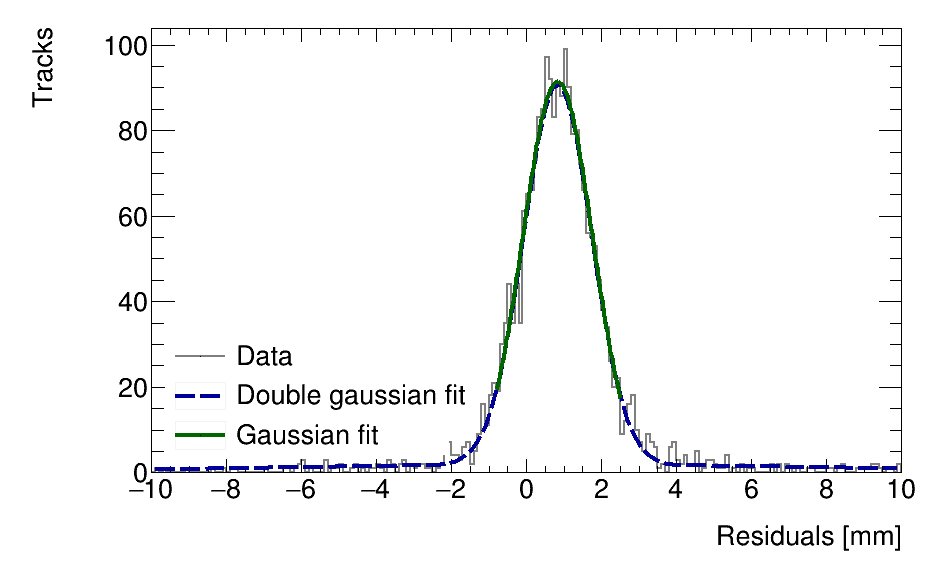
\includegraphics[width = \textwidth]{figures/figure_double_gaussian_quick_and_dirty_2900V_log_scale_gaussian_QL2C04_2900V_2021-02-08_2_xbin_10_ybin_5_100mm.png}
    \caption{Residual distribution for tracks on layer 1 built from hits on layers 3 and 4 for $x\in\left[-3.00, 97.00\right],  y\in\left[394.60, 494.60\right] mm$ for QL2.C.4 fit with a double gaussian and a single gaussian in a range of $\pm$1 RMS from the histogram mean.}
    \label{fig:double_gaussian_example_fit}
\end{figure}

For all residual distributions in \SI{100}{\milli\meter} by \SI{100}{\milli\meter} bins on layer 1 built from hits on layers 3 and 4, the difference in gaussian and double gaussian means and $\sigma$'s is shown in figure \ref{fig:double_gaussian_compare_fits}. Since the RMS of the residual mean differences distribution is less than \SI{50}{\micro\meter} the gaussian fit gave the same result within the required precision. Moreover, this is for the tracking combination with the worst extrapolation lever arm and the widest distribution of mean differences; the interpolation combinations have narrower distributions. 

The gaussian $\sigma$ should be larger than the double gaussian $\sigma$ because the gaussian distribution includes the effect of the noise tracks with large residuals, while the double gaussian models signal and background residuals separately. For this analysis, only the residual mean was important, so the systematic overestimate of the signal $\sigma$ in the gaussian fit shown on the right of figure \ref{fig:double_gaussian_compare_fits} was allowed.

\begin{figure}
    \centering
    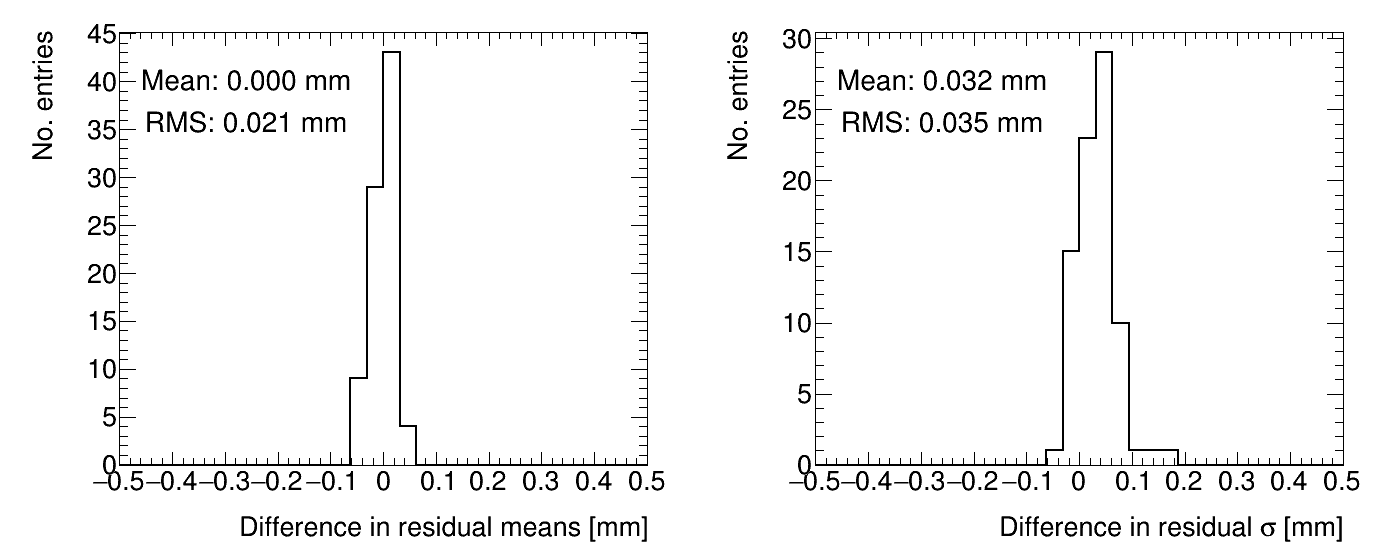
\includegraphics[width = \textwidth]{figures/figure_compare_residual_fits_QL2C04_2900V_2021-02-08_2_fit_range_mean_pm_RMS_minus_quick_and_dirty_2900V_log_scale_layer1_fixedlayers34.png}
    \caption{Difference in residual distribution means and $\sigma$'s for a gaussian and double gaussian fit, for all residual distributions in \SI{100}{\milli\meter} by \SI{100}{\milli\meter} bins on layer 1 built from hits on layers 3 and 4 for QL2.C.4, data taken at 2900 V.}
    \label{fig:double_gaussian_compare_fits}
\end{figure}

% --------------------------------------------------
\section{Area of residual distribution regions of interest}
% --------------------------------------------------
\label{appendix:systematics_bin_size}
% Edit count: 1

% DO I NEED TO EXPLAIN THIS IN MATH? I tried on June 3rd in my notes, it's complicated for such a simple thing.
% If this flies, you'll need to establish that reference frame == two fixed layers' frame as jargon in your thesis.
% Also need to establish x == perpendicular to wires; y == perpendicular to strips. ==> How do I do this consistently?
% May need to add 3100V reference if it's not already defined in your thesis.
% Define ROI as short form?

%TODO : How do I cite the distribution of rotations angles by Dylan?
The area of the region of interest in which to include tracks is primarily motivated by the misalignment model: the width of the region should be less than the scale on which the local offset is expected to change significantly. Changes in offset of order \SI{50}{\micro\meter}, the approximate position resolution of the sTGCs in the $\eta$-coordinate, are significant. In a misalignment model with an offset and rotation, only the rotation changes the local offset with respect to the x-coordinate \footnote{The effect of rotation can be modeled by assuming the recorded track position is related to the hit position by a passive rotation. The angle of rotation is the relative angle between the layer of interest and the nominal geometry. The local offset does change with respect to the track's y coordinate as well, but negligibly in the limit of small rotation angles.}.  The distribution of the as-built cathode board rotation angles shows that the RMS of the rotation angle is \SI{200}{\micro\radian} [https://indico.cern.ch/event/1035057/ PG. 18]; however, the distribution has a long tail so a typical rotation angle of \SI{1000}{\micro\radian} was used here. A rotation of \SI{1000}{\micro\radian} will cause a \SI{50}{\micro\meter} change in local offset over a change in x of \SI{50}{\centi\meter}. Therefore, the width of the region of interest should be less than \SI{500}{\milli\meter}.

Two other factors inform the width of the region. First, since the hits' x-coordinates are discrete the width in x must be larger than the pitch of the wire groups to ensure the bin will have a sufficient number of tracks fall in it. Second, more tracks will be included in a larger area so more statistics will be available for the residual distribution fit. For the bin widths wider than two wire groups, the statistics are sufficient. For each x-ray residual, the mean cosmics residual was calculated for a few different bin widths, and the difference in means plotted. Figure \ref{fig:area_bin_size_mean_diff} shows an example for QL2.C.4. The width of the distribution is on the order of \SI{50}{\micro\meter}, showing that the calculation of the residual mean is relatively robust with respect to the area of the bin. However, \SI{50}{\micro\meter} is greater than the typical statistical uncertainty on the cosmic residual of means, which ranges from \SI{10}{\micro\meter} - \SI{40}{\micro\meter} depending on the tracking combination under study. Therefore, the cosmic residual means are assigned an uncertainty of \SI{50}{\micro\meter}.
%TODO : Verity that you actually apply the 50 um uncertainty.

%TODO : This figure should have the mean and rms on it.

\begin{figure}
    \centering
    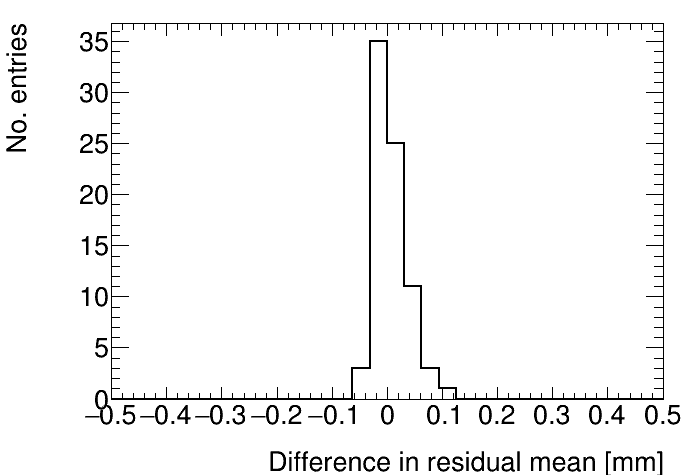
\includegraphics[width = \textwidth]{figures/compare_residual_fits_around_xrays_QL2C04_3100V_2021-05-20_100mm_width_bins_minus_QL2C04_3100V_2021-06-02_200mm_width_bins_means_difference.png}
    \caption{Difference in cosmic residual means around x-ray residuals for square bins of 100 mm width and 200 mm width for QL2.C.4.}
    \label{fig:area_bin_size_mean_diff}
\end{figure}

For this analysis, \SI{100}{\milli\meter} by \SI{100}{\milli\meter} by \SI{100}{\milli\meter} bins were used.

% --------------------------------------------------
\section{Differential non-linearity}
% --------------------------------------------------
\label{appendix:systematics_dnl}
% Edit count: 1
In this context, differential non-linearity (DNL) is when the reconstructed cluster mean is biased by the fit of the discretely sampled PDO distribution over the strips. The bias depends on the relative position of the avalanche with respect to the center of the closest strip. For a summary of DNL, refer to page 40 of Lefebvre's thesis \cite{lefebvre_thesis}. The cluster mean was corrected for DNL using the equation:

\begin{equation}
\label{eqn:dnl_corr}
y' = y + a \sin \left( 2 \pi y_{rel} \right)
\end{equation}

where $y$ is the cluster mean, $y_{rel}$ is the relative position of the cluster mean with respect to the strip's center, $a$ is the amplitude of the correction, and $y'$ is the corrected cluster mean. The amplitude can be derived by comparing the reconstructed hit position to the expected hit position, as done in Abusleme, 2016 \cite{abusleme_performance_2016}. With cosmic muons, there is no reference hit position to compare to, so track residuals were used as a proxy \cite{lefebvre_thesis}. The hallmark of the DNL effect is the periodic pattern in the residual versus $y_{rel}$ profile, and the effect of correcting the cluster means using an amplitude of \SI{50}{\micro\meter} is shown in figure \ref{fig:dnl_corr_effect}. An amplitude of \SI{50}{\micro\meter} was based on Lefebvre's estimate of the DNL amplitudes by layer, quadruplet and cluster size using exclusive cosmic muon tracks in \package{tgc\_analysis/CosmicsAnalysis}. Little variation was seen in the amplitude parameters with respect to the quadruplet tested, the layer and the cluster size so a universal correction was used.
%TODO How little is little? Check your notes.
%TODO exclusive better be defined somewhere clearly.

\begin{figure}
    \centering
    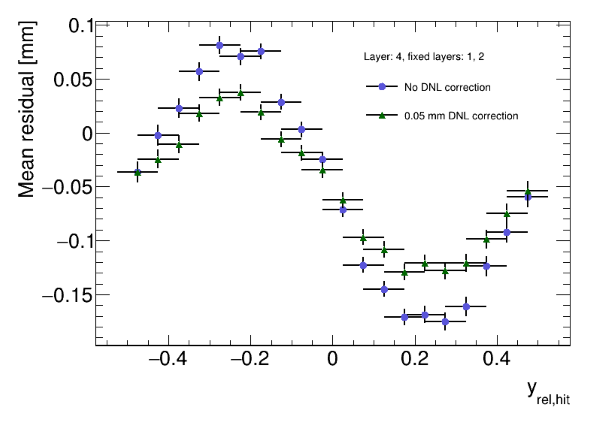
\includegraphics[width = \textwidth]{figures/figure_dnl_profiles_blue_QL2P08_3100V_2021-06-18_no_dnl_green_QL2P08_3100V_2021-06-18_2_50um_universal_DNL_layer4_fixed12.png}
    \caption{Effect applying a \SI{50}{\micro\meter} DNL correction to the cluster means on the residual vs $y_{rel}$ distribution for tracks built from layers 1 and 2 and extrapolated to layer 4 for QL2.P.8.}
    \label{fig:dnl_corr_effect}
\end{figure} 

Although the correction is not large enough in this case, the figure shows that the correction does reduce the DNL effect. Slightly better performance is seen in the interpolation tracking combinations where the quality of the residuals is better. DNL corrections for cosmic muon data are difficult because the DNL effect is obscured by the effect of misalignments and noise. Misalignments cause the center of the sine pattern in figure \ref{fig:dnl_corr_effect} to be shifted off of zero, since the mean of residuals is shifted.

In figure \ref{fig:dnl_compare_fits}, it is apparent that the effect of the DNL correction on the mean of the residual distribution in \SI{100}{\milli\meter} by \SI{100}{\milli\meter} areas is on the order of micrometers in the worst extrapolation case. Although the $\sigma$'s of the residual distributions shrink with the DNL correction, the mean is the parameter of interest. Therefore, for this analysis DNL was not corrected for.

\begin{figure}
    \centering
    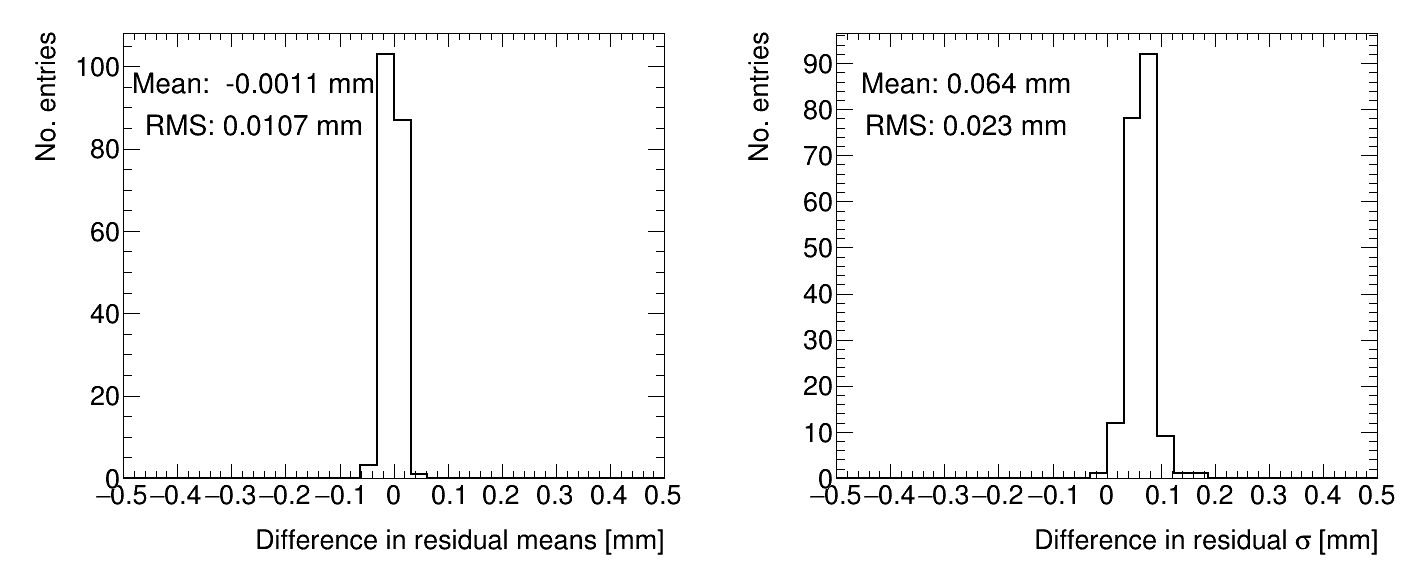
\includegraphics[width = \textwidth]{figures/figure_compare_residual_fits_QL2P08_3100V_2021-06-18_no_dnl_minus_QL2P08_3100V_2021-06-18_2_50um_universal_DNL_layer4_fixedlayers12.png}
    \caption{Difference in residual distribution means and $\sigma$'s with and without DNL correction for residuals on layer 4 from reference layers 1 and 2 for QL2.P.8.}
    \label{fig:dnl_compare_fits}
\end{figure}

The $\sigma$'s of the residual distributions do shrink with the DNL correction but not so much to affect the residual means, which are the important parameter for this analysis. Therefore, since the effect of the DNL correction is negligible, it was not pursued further.






























